\documentclass[a4paper,twoside,titlepage]{article}

%--- Packages ----------------------------------------------------------------
\usepackage{a4}
\usepackage[english]{babel}
\addto\extrasswedish{%
	\def\sectionautorefname{Avdelning}%
	\def\subsectionautorefname{Underavdelning}%
	\def\figureautorefname{Figur}%
	\def\tableautorefname{Tabell}%
}
\addto\extrasenglish{%
	\def\outputautorefname{Output}%
}
\usepackage[inner=2cm,top=2cm,outer=3cm,bottom=1cm,includehead,includefoot]{geometry}
\usepackage[utf8]{inputenc}
\usepackage{moreverb}
\usepackage{float}
\usepackage{graphicx}
%\usepackage{makeidx}
%\makeindex
% Don't forget to run makeindex and include \printindex
\usepackage{fancyhdr}
\usepackage[colorlinks=true,linkcolor=magenta,urlcolor=blue]{hyperref} % Reference by title

\setcounter{tocdepth}{2} % Only subsections in toc

%--- Definitions -------------------------------------------------------------

\def\author			{Emil Eriksson}
\def\email			{c07een@cs.umu.se}
\def\course			{Embedded Systems}
\def\coursename	{Assignment 1}
\def\delivery		{Report}
\def\version		{1.0}
\def\trivialname	{Radio Controlled Car}
\def\tutor			{}


% New output float
\floatstyle{boxed}
\newfloat{program}{thp}{lop}
\floatname{program}{Program}
\newfloat{output}{thp}{lop}
\floatname{output}{Output}

%\restylefloat{figure}

\hypersetup{
pdfauthor = {\author},
pdftitle = {\trivialname{} - \delivery},
pdfsubject = {\coursename},
pdfkeywords = {umu, edu, mips, manual}
}


\newcommand{\HUGE}{\fontsize{36}{42}\selectfont{}}
\newcommand{\helvetica}{\fontfamily{phv}\selectfont}
\newcommand{\degree}{\ensuremath{^\circ}}
\pagestyle{fancy}
	\lhead[\coursename]{\today}
	\chead[\textsc{\trivialname~- \delivery~\version}]{\textsc{\trivialname~- \delivery~\version}}
	\rhead[\today]{\course}
	
	\lfoot[\thepage]{\author}
	\cfoot[]{}
	\rfoot[\email]{\thepage}
	
	\renewcommand{\headrulewidth}{0.4pt} 
	\renewcommand{\footrulewidth}{0.4pt}

%-----------------------------------------------------------------------------
\begin{document}
\pagestyle{empty}
%--- Titlepage ---------------------------------------------------------------
\begin{titlepage}
	{
	\helvetica
	\begin{flushright}
		\small \coursename{} \course\\
	\end{flushright}
	\begin{center}
		\LARGE \trivialname\\
		\HUGE { \textbf{\delivery}} \\
		\small \author{} (\href{mailto:\email}{\email})\\
		\normalsize \textbf{Version \version}\\
		\vspace{155mm}
	\end{center}
	}
	\begin{flushright}
		\subsection*{Examinator}
		Nils-Erik Eriksson \href{mailto:nilserik.eriksson@tfe.umu.se}{nilserik.eriksson@tfe.umu.se}
	\end{flushright}
\end{titlepage}

\pagestyle{fancy}
\pagenumbering{roman}
%--- Table of contents -------------------------------------------------------
\tableofcontents
\listoffigures
%\clearpage
\newpage

%--- Document ----------------------------------------------------------------
\pagenumbering{arabic}

%-----------------------------------------------------------------------------
\section{Introduction} % (fold)
\label{sec:introduction}

\subsection{Goal} % (fold)
\label{sub:goal}
% subsection goal (end)

\subsection{Usage} % (fold)
\label{sub:usage}
% subsection usage (end)

% section introduction (end)

%-----------------------------------------------------------------------------
\section{Materials and methods} % (fold)
\label{sec:materials_and_methods}

\subsection{Microcontroller} % (fold)
\label{sub:microcontroller}
% subsection microcontroller (end)

\subsection{Tranciever} % (fold)
\label{sub:tranciever}
% subsection tranciever (end)

\subsection{Communication} % (fold)
\label{sub:communication}
% subsection communication (end)

\subsection{IR-sensor} % (fold)
\label{sub:ir_sensor}
% subsection ir_sensor (end)
% section materials_and_methods (end)

\section{Evaluation} % (fold)
\label{sec:evaluation}
% section evaluation (end)

\begin{figure}[hp]
   \caption{Circuit diagram of the radio controlled car.}
   \label{fig:circuit}
   \vspace{15mm}
   \centering
      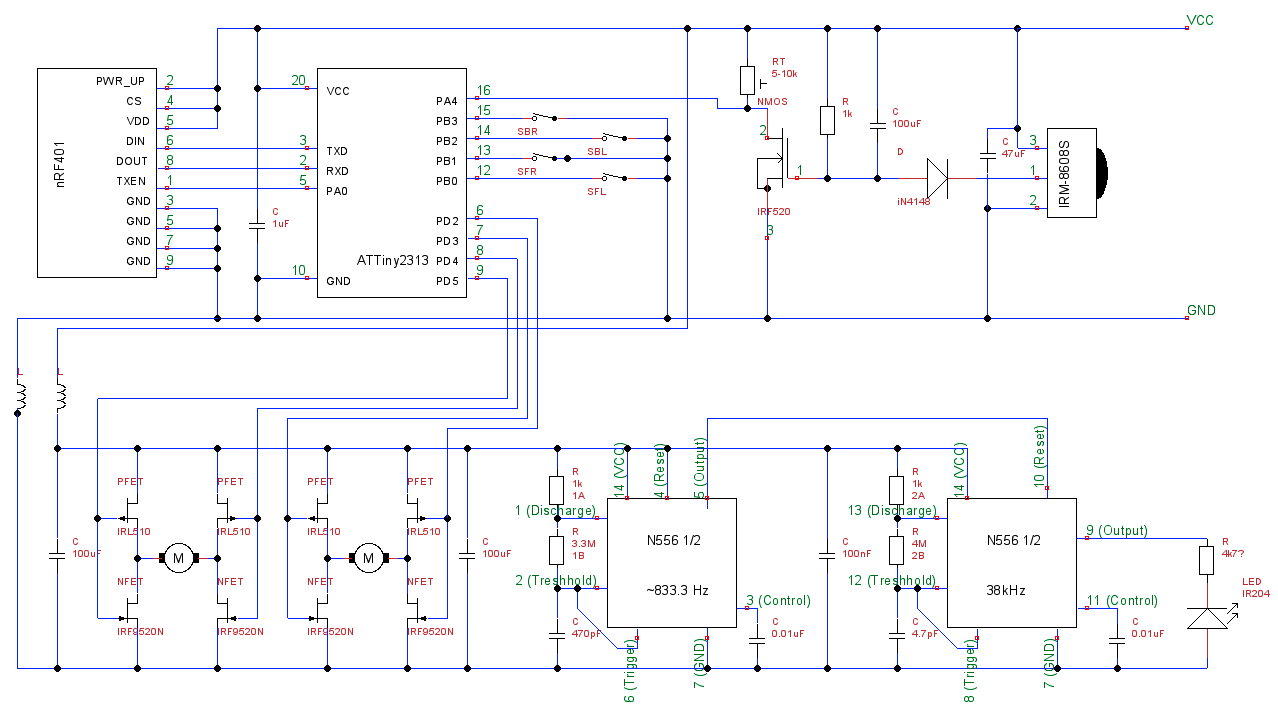
\includegraphics[angle=90,height=0.8\textheight]{tCad1.pdf}
\end{figure}

% \clearpage
% \appendix
% \newpage

\end{document}